\resetNumActivite{}
\section{Travail à réaliser}
\UPSTIinfo[Variables d'entrées utiles et adresses DALI]{
    \label{info:var}
    \begin{minipage}{.5\textwidth}
    \begin{tabular}{|c|c|}
        \hline
        \textbf{Element} & \textbf{Nom de variable}\\\hline
        Bouton arret urgence & ixArretUrgence\\
        Bouton poussoir Blanc & ixBpAcq \\\hline
        Bouton poussoir Rouge & ixBpRouge \\
        Bouton poussoir Vert & ixBpVert \\
        Bouton poussoir Bleu & ixBpBleu \\\hline
        Sélecteur Haut & ixSelUp \\
        Sélecteur Bas & ixSelDown \\\hline
    \end{tabular}
\end{minipage}\hfill
\begin{minipage}{.5\textwidth}
    \begin{flushright}
    \begin{tabular}{|l|c|}
        \hline
        \textbf{Element DALI} & \textbf{Adresse DALI}\\\hline
        \multirow{4}{4cm}{Luminaires (de la fenêtre vers le couloir)} & 1 \\
        & 2 \\
        & 3 \\ 
        & 4 \\\hline
        {Lampe Rouge} & 10 \\
        {Lampe Verte} & 11 \\
        {Lampe Bleue} & 12 \\
        \hline
    \end{tabular}
\end{flushright}
\end{minipage}
}
\subsection{Observation matérielle}
\begin{UPSTIactivite}[][Elements du système]
    \label{act:tpElts}
    \UPSTIquestion{Noter la référence de votre automate et repérer le coupleur DALI (750-641) sur votre maquette.}
\end{UPSTIactivite}

\subsection{Configuration du projet}
\begin{UPSTIactivite}[][Préparation du projet]
    \UPSTIetape{Lancer la machine virtuelle \textit{ARS (Win10)}}
    \UPSTIetape{Pendant qu'elle démarre : Sous votre répertoire associé à ce module, copier le squelette de l'application \textbf{correspondant à l'automate de votre plateforme} qui se trouve sous \\ \textbf{U:\textbackslash Documents\textbackslash BUT\textbackslash GEII\textbackslash ModuleS3\textbackslash R3.13 Réseaux Spécialisés EME \textbackslash Squelettes \textbackslash Dali}. }
    \UPSTIetape{Lancer le logiciel \textbf{CoDeSys V2.3} sur la machine virtuelle et ouvrir le squelette de l'application.}

    Nous allons à présent inclure la bibliothèque DALI\_02.lib dans notre projet afin de pouvoir utiliser les blocs fonctionnels nécessaires à la communication avec le bus DALI.
    
    \UPSTIetape{Dans l'onglet \textbf{Ressources}, ouvrir le \textbf{Gestionnaire de bibliothèques}. Faire un clic droit pour ajouter une bibliothèque et sélectionner \textbf{DALI\_02.lib}. }
    Elle se trouve dans le répertoire \textbf{C:\textbackslash Program Files\textbackslash WAGO Software\textbackslash CoDeSys V2.3\textbackslash Targets\textbackslash WAGO\textbackslash Librairies\textbackslash Building}

    \begin{center}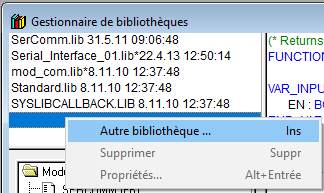
\includegraphics[width=.3\textwidth]{insererBibliotheque} \hspace{1cm}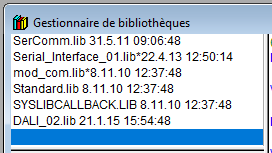
\includegraphics[width=.3\textwidth]{ajoutBibliothequeDALI}
    \end{center}
\end{UPSTIactivite}


\subsection{Premières commandes DALI}
Dans cette section, nous allons mettre en place notre première communication DALI. Nous allons commander un plafonnier à partir d'un bouton poussoir en utilisant un bloc fonction de la bibliothèque DALI\_02.lib.
\begin{UPSTIactivite}[][Définition des types de données]
    \UPSTIetape{Dans l'onglet \textbf{Type de données}, renseigner le type \textbf{CDaliJobList} (Préparation \ref{act:fbDALIJoblist})}
\end{UPSTIactivite}

\begin{UPSTIactivite}[][Programme bloc Fonction]
    \UPSTIetape{Ajouter un nouveau module : 
    \begin{itemize}
        \item Dans l'onglet \textbf{Modules}, ajouter un nouveau module (\textit{Clique-droit -> Insérer objet})
        \item Le nommer \textit{Plafonniers} et langage CFC. L'appeler dans le programme DALI
        \end{itemize}}
    \UPSTIetape{Dans ce nouveau programme, déclarer la variable \textbf{jobList} de type \textbf{CDaliJobList} \textit{(Tutoriel \ref{tuto:declarationAutomatique})}
        \begin{itemize}
            \item Donner la valeur par défaut \textbf{1} à la variable \textbf{m\_bModule\_750\_641} \textit{(Numéro du module DALI)}
        \end{itemize}}
    \UPSTIetape{Appeler \textit{(Placer)} le bloc fonction \textbf{jobList.m\_fbDALI\_Joblist} (Préparation \ref{prepa:fbDALIJoblist}, Tutoriel~\ref{tuto:insertionBloc}).}
    \UPSTIetape{Déclarer un Fonction bloc \textbf{FbDALI\_LatchingRelay} et l'insérer. \textit{(Prépa \ref{prepa:telerupteur}, Tuto~\ref{tuto:declarationAutomatique}, Tuto~\ref{tuto:insertionBloc}) .}}
    \UPSTIetape{Faire vérifier et tester votre programme.}
\end{UPSTIactivite}

\UPSTItuto[Déclaration automatique dans CoDeSys]{%
\label{tuto:declarationAutomatique}
    Dans le logiciel CoDeSys, il est possible de déclarer automatiquement des variables dont le type a été préalablement défini. Par exemple, pour déclarer une variable de type \textbf{CDaliJobList} : 
    \begin{enumerate}
        \item Clique-droit sur une ligne vide 
        \begin{itemize}
            \item \textit{Déclarer automatiquement}
        \end{itemize}
        \item Cliquer sur les $\dots$ de \textbf{Type} : 
        \begin{itemize}
            \item Type défini
            \item Sélectionner le type \textit{(CDaliJobList, par exemple)}
        \end{itemize}
        \item Cliquer sur les $\dots$ de \textbf{Valeur initiales} : 
        \begin{itemize}
            \item Définir les valeurs initiales pertinentes \textit{(Celles qui ne seront pas impérativement définies dans le programme, par exemple.)}
        \end{itemize}
        \item Donner un nom à la variable dans le champs \textbf{Nom}
    \end{enumerate}
    \begin{center}
        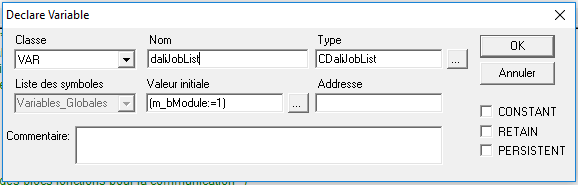
\includegraphics[width=.75\textwidth]{declarationAutomatique_menu}
    \end{center}
}%

\UPSTItuto[Insertion d'un bloc fonction]{
    \label{tuto:insertionBloc}
    Pour insérer un bloc fonction dans un programme CFC : 
    \begin{enumerate}
        \item Cliquer sur l'icone Module 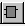
\includegraphics[height=10pt]{tuto/iconeModule}
        \item Descendre la souris dans la zone de bloc
        \item Renommer le bloc \textit{AND} par le type de bloc que vous voulez insérer (\textit{fbDALI\_Joblist}, par exemple)
        \\\begin{center}
            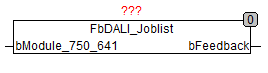
\includegraphics[clip, trim= 1mm 5mm 1mm 1mm,height=1.2cm]{tuto/blocVierge}
        \end{center}
        A cette étape, le bloc est inséré, mais n'est pas encore appelé. Il faut lui associer une variable déclarée. 
        \item Double-cliquer sur les \textcolor{red}{\textbf{???}} et lui associer une variable existante. 
        \\\begin{center}
            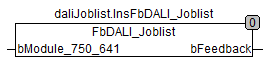
\includegraphics[clip, trim= 1mm 3mm 1mm 1mm,height=1.2cm]{tuto/blocOk}
        \end{center}
        \item Ajouter une entrée (
\includegraphics[height=10pt]{tuto/iconeEntree}) et une sortie (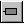
\includegraphics[height=10pt]{tuto/iconeSortie}) puis leur associer une variable ou une valeur. 
        \\\begin{center}
            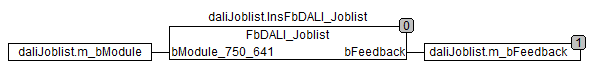
\includegraphics[clip, trim= 1mm 3mm 1mm 3mm,height=1.2cm]{tuto/blocComplet}
        \end{center}
    \end{enumerate}
}
\vspace{-.8cm}
\begin{UPSTIactivite}[][Appel d'un bloc en ST]
    Dans cette activité, nous allons réaliser la même chose mais en appelant les blocs fonction en langage ST. Cela nous permettra, par exemple, de créer plusieurs instances à l'aide d'une boucle \textit{for} et de tableaux. 
    \UPSTIetape{Dans le programme DALI : }
    \begin{itemize}
        \item Déclarer une variable \textbf{bLatchingRelay} de type \textbf{FbDALI\_LatchingRelay} \textit{(Tutoriel \ref{tuto:declarationAutomatique})}
        \item Appeler le bloc fonction en ST (Tutoriel \ref{tuto:aideSaisie}) et lui associer les valeurs d'entrées et sorites.
        \item Faire vérifier et tester votre programme.
    \end{itemize}
    %\UPSTIetape{Faire de même avec un tableau de 3 blocs fonction \textbf{FbDALI\_LatchingRelay} et les appeler dans une boucle \textit{for}.}
\end{UPSTIactivite}


\vspace{-1cm}

\UPSTItuto[Aide à l'appel d'élément déclaré]{
    \label{tuto:aideSaisie}
    Dans le logiciel CoDeSys, il est possible d'utiliser une variable définie ou d'appeler une fonction ou un bloc fonction déclaré facilement en suivant les étapes suivantes :
    \begin{itemize}
        \item Clique droit sur une ligne vide
        \begin{itemize}
            \item \textit{Liste de sélection pour l'édition}
        \end{itemize} 
        \item Chercher l'élément que vous souhaitez appeler 
    \end{itemize}
    \begin{center}
        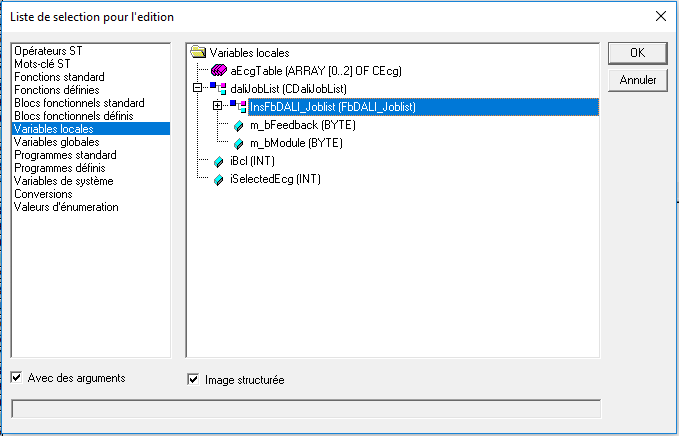
\includegraphics[width=.7\textwidth, clip,trim=0mm 55mm 0mm 0mm]{aideSaisie_menu}
    \end{center}
}


\subsection{Envoi de commandes plus complexes}

\begin{UPSTIactivite}[][Mise en place de la communication avec le ballast Rouge]
    \UPSTIetape{Définir la structure de données \textbf{CEcg} (Préparation \ref{act:fbDALIMaster})}
    \UPSTIetape{Déclarer une variable \textbf{ecgRouge} de type \textbf{CEcg} (Tutoriel \ref{tuto:declarationAutomatique})}
    \UPSTIetape{Insérer le bloc fonction \textbf{FbDALI\_Master} associé. \textit{(Tuto~\ref{tuto:aideSaisie}) .}} et lui associer les membres de sa structure.
\end{UPSTIactivite}

\UPSTIremarque[Qu'avons-nous fait jusque là ?]{
    Les étapes précédentes ont permis de déclarer les variables et les blocs fonctionnels nécessaires à la mise en place d'un bus DALI.

    Le bloc fonction \textbf{fbDALI\_Master} scrute sa variable d'entrée \textbf{xStartDaliMaster} dans l'attente d'une mise à 1. Lorsque cela se produit, il exécute la commande DALI paramétrée sur ses autres entrées. Pour simplifier l'accès à ses variables d'entrées et de sortie, nous avons créé une classe \textbf{CEcg} et associé les attributs de cette classe aux entrées du bloc. 

    Le bloc fonction \textbf{fbDALI\_Joblist} se chargera d'envoyer les commandes que les blocs \textbf{fbDALI\_Master} auront généré. Pour simplifier l'accès à ses variables d'entrées et sorties, nous avons créé une classe \textbf{CDaliJobList} et associé les attributs de cette classe aux entrées du bloc.
}

\begin{UPSTIactivite}[][Commande directe]
    \UPSTIetape{Écrire un programme qui allume la lampe rouge à 75\% de sa luminosité maximale lorsque le bouton rouge est appuyé et qui l'éteint lorsque le bouton est relâché.} Faire vérifier par l'enseignant.
\end{UPSTIactivite}

\UPSTIattention{Si le programme précédent est fait trop simplement, des commandes DALI sont envoyées sans arrêt, saturant le réseau DALI. Il faut corriger cela en utilisant, par exemple, la détection de front montant.}

\begin{UPSTIactivite}[][Correction du programme précédent]
    \UPSTIetape{Si nécessaire, corriger le programme précédent pour n'envoyer qu'une seule commande DALI à chaque changement d'état.}
\end{UPSTIactivite}

\pagebreak
\section{Programmes avancés}

\UPSTIboiteCentrale{Un bouton par couleur}{
    \begin{itemize}
        \item Le bouton poussoir rouge commande la lampe rouge.
        \item Le bouton poussoir vert commande la lampe verte.
        \item Le bouton poussoir bleu commande la lampe bleue.
    \end{itemize}
}

\UPSTIboiteCentrale{Cahier des charges : Intensité lumineuse}{
    \begin{itemize}
        \item Le sélecteur 3 position modifie l'intensité de la lampe rouge
    \end{itemize}}


\begin{UPSTIactivite}
    \UPSTIetape{Programmer le cahier des charges \textit{Un bouton par couleur}. Tester le programme}
    \UPSTIetape{Programmer le cahier des charges \textit{Intensité lumineuse}. Tester le programme}
\end{UPSTIactivite}

\UPSTIboiteCentrale{Cahier des charges : Sélection de couleur}{
    \begin{itemize}
        \item Chaque bouton de couleur permet de sélectionner la couleur de la lampe à commander.
        \item Le sélecteur à 3 boutons permet d'augmenter ou de diminuer l'intensité lumineuse de la lampe sélectionnée.
    \end{itemize}}

\begin{UPSTIactivite}
    Pour coder le cahier des charges ci-dessus, on propose la stratégie suivante : 
    \UPSTIetape{Supprimer les instances CEcg créer et les remplacer par un tableau de 3 instances de CEcg, un par couleur.}
    \UPSTIetape{Rassembler les appels des blocs \textbf{FbDALI\_Master} dans une boucle \textit{for}. \textit{Pour cela, il faudra créer un tableau}}
    \UPSTIetape{Modifier le reste du programme pour respecter le Cahier des charges.}
    \UPSTIetape{Tester et faire vérifier votre programme}

\end{UPSTIactivite}

\begin{UPSTIactivite}[][Appeler l'enseignant]
    \vspace{4cm}
\end{UPSTIactivite}

